%! BibTeX Compiler = biber

\documentclass[chapterprefix,a4paper,
openany,
10pt,
reqno, 
bibliography=totoc,listof=totoc,index=totoc,%
fleqn,twoside]{book}

\usepackage[T1]{fontenc}
\usepackage[utf8]{inputenc}
\usepackage[backend=biber]{biblatex} %Imports biblatex package
\usepackage{todonotes}
\usepackage{xcolor}
%\usepackage[toc, acronym, automake]{glossaries}
\usepackage{listings}
\usepackage{graphicx} % Required for inserting images
\usepackage{hyperref} % https://www.overleaf.com/learn/latex/Hyperlinks#Styles_and_colours
\usepackage{fancyhdr}

\usepackage[
	left=3.5485cm,
	right=2.5485cm,
	top=3.5cm,	
	bottom=2.7cm,
	footskip=1.5cm
]{geometry}

% For Listing 
\usepackage{listings}
\usepackage{xcolor}

\lstdefinestyle{mypicturestyle}{
  language=Java,
  basicstyle=\ttfamily\small,
  numbers=left,
  numberstyle=\tiny\color{gray},
  stepnumber=1,
  numbersep=10pt,
  frame=single,
  rulecolor=\color{black},
  frameround=tttt,
  xleftmargin=1.2em,
  framexleftmargin=1.2em,
  breaklines=true,
  showstringspaces=false,
  tabsize=4,
  captionpos=b,
  keywordstyle=\color{blue},
  commentstyle=\color{green!50!black},
  stringstyle=\color{orange!70!black}
}
\usepackage{titlesec}
\newcommand{\hsp}{\hspace{25pt}}
\newcommand{\lineindent}{\hspace*{0.4cm}}


%%%%%%%%%%%%%%%%%%%%%%%%%%%%%
% chapter header and footer
%%%%%%%%%%%%%%%%%%%%%%%%%%%%%
\pagestyle{fancy}
\fancyhead[LE]{\leftmark}
\fancyhead[LO,RE]{}
\fancyhead[RO]{\rightmark}
\fancyfoot[CE,CO]{}
\fancyfoot[LE,RO]{\thepage}
\renewcommand{\headrulewidth}{0.5pt}


%%%%%%%%%%%%%%%%%%%%%%%
% chapter titles
%%%%%%%%%%%%%%%%%%%
\titleformat
{\chapter}
	{\Large\bfseries}	% format
	{ \textsl{\textcolor{gray}{Chapter \thechapter}}\hsp \vspace{1ex} } 	% label
	{1.1ex} 			% sep	
	{ \noindent\filright }
%%%%%%%%%%%%%%%%%%%%%%%

\graphicspath{{figures/}}

\hypersetup{
	colorlinks=true,
	linkcolor=blue,
	citecolor=blue
}


\bibstyle{alpha}
\addbibresource{references.bib} %Import the bibliography file

%% glossaries
%\makeglossaries
%
%\newglossaryentry{test}
%{
%	name=testEntry,
%	description={This is a test entry for testing glossaries}
%}



\renewcommand{\chapterautorefname}{Chapter}
\renewcommand{\sectionautorefname}{Section}
\renewcommand{\subsectionautorefname}{Section}
\renewcommand{\subsubsectionautorefname}{Section~\thesubsection,}
\def\subfigureautorefname{Figure}
\def\figureautorefname{Figure}

\newcommand{\todoi}[1]{\todo[inline]{#1}}
\newcommand{\defineReviewCommands}[2]{
	\expandafter\def\csname#1\endcsname##1{\todo[color=#2]{##1 -#1}}%%%
	\expandafter\def\csname#1i\endcsname##1{\todo[inline,caption={},color=#2]{##1 -#1}}%%%
}

\defineReviewCommands{sg}{blue!20}



\title{Analysis of Real-World Developer Mistakes 
in configurable software systems}
\author{Salma Khair}
\date{01 January 2026}

%\addbibresource{references.bib} %Import the bibliography file
\usepackage{subfiles} % Best loaded last in the preamble

\begin{document}

    \pagenumbering{roman}
    \begin{titlepage}

\newcommand{\HRule}{\rule{\linewidth}{0.5mm}} % Defines a new command for the horizontal lines, change thickness here
%----------------------------------------------------------------------------------------

\center % Center everything on the page

%----------------------------------------------------------------------------------------
%	LOGO SECTION
%----------------------------------------------------------------------------------------


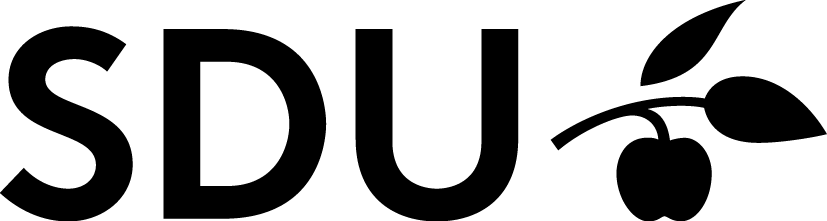
\includegraphics[width=6cm]{title/SDU_BLACK.png}\\[1cm] % Include a department/university logo - this will require the graphicx package
 
%----------------------------------------------------------------------------------------
%	HEADING SECTIONS
%----------------------------------------------------------------------------------------

\textsc{\LARGE University of Southern Denmark}\\[1.5cm] % Name of your university/college
\textsc{\Large Bachelor Project}\\[0.5cm] % Major heading such as course name
\textsc{\large IMADA}\\[0.5cm] % Minor heading such as course title

%----------------------------------------------------------------------------------------
%	TITLE SECTION
%----------------------------------------------------------------------------------------
\makeatletter
\HRule \\[0.4cm]
{ \huge \bfseries \@title}\\[0.4cm] % Title of your document
\HRule \\[1.5cm]
 
%----------------------------------------------------------------------------------------
%	AUTHOR SECTION
%----------------------------------------------------------------------------------------

\begin{minipage}{0.4\textwidth}
\begin{flushleft} \large
\emph{Student:}\\
\@author\\[1.2em] % Your name
%\emph{Student:} \\
% 	%second name
\end{flushleft}
\end{minipage}
~
\begin{minipage}{0.4\textwidth}
\begin{flushright} \large
\emph{Supervisor:} \\
Dr. rer. nat. Sandra Greiner 
Associate Professor \\
\end{flushright}
\end{minipage}\\[2cm]
\makeatother

% If you don't want a supervisor, uncomment the two lines below and remove the section above
%\Large \emph{Author:}\\
%John \textsc{Smith}\\[3cm] % Your name

%----------------------------------------------------------------------------------------
%	DATE SECTION
%----------------------------------------------------------------------------------------

{\large \today}\\[2cm] % Date, change the \today to a set date if you want to be precise

\vfill % Fill the rest of the page with whitespace

\end{titlepage}

    \tableofcontents

    \setlength{\parskip}{\baselineskip}
    \setlength{\parindent}{0pt}

    \clearpage
    \pagenumbering{arabic}
    \setcounter{page}{1}

	\begingroup
		\pagestyle{fancy}
	  	\chapter{Introduction}
\label{chp:intro}

% Answer the following question

% What is the context of your thesis?  What area of computer science is it located in?
% What is the problem that you are addressing?
% How do you try to solve the problem? -> implement a Rust adapter for ECCO
% How do you evaluate your solution? -> 
% What is the result of your evaluation?
% How is the thesis structured in the following?
Modern software systems are rarely developed as a single, fixed program.  
Instead, many systems are configurable, meaning that the same code base can be
compiled into different software variants depending on hardware, platform, or
selected features.
A common way to implement such configurability is through conditional code
guarded by presence conditions, for example using preprocessor directives such
as \texttt{\#if} and \texttt{\#ifdef}.  
Presence conditions determine in which configurations a particular code fragment
is included and therefore directly influences the behavior of the resulting
software variants.

This bachelor thesis is situated in the area of software engineering, with a
focus on configurable software systems and variability analysis.
It studies how changes to conditional code, such as presence conditions
e.g. \texttt{\#ifdef}, affect software systems over time by analysing large
software repositories.
In standard version control systems, changes are represented as textual diffs
that show added or removed lines of code.  
While this representation is sufficient for many development tasks, it is often
insufficient for configurable systems.  
In such systems, even a small textual change can have a large semantic impact if
it modifies a presence condition.

For example, a minor edit to a conditional expression may silently expand or
restrict the set of configurations in which a code fragment is active.  
These effects are not visible in standard diffs and are often undocumented in
commit messages.  
As a result, developers and tools may overlook unintended changes to variability,
which can lead to configuration of specific faults that are difficult to detect.
The problem addressed in this thesis is therefore the limited ability of
traditional diffs to explain the impact of changes to presence conditions.  
In particular, the thesis investigates how developer mistakes related to
variability can be identified by analyzing commits at the level of variability
semantics rather than raw text differences.

To address this problem, this thesis builds on the DiffDetective tool to explicitly
identify changes in variability. 
DiffDetective analyzes software evolution by mapping source code and annotations
to structured representations and by classifying edits according to their effect
on variability.  
Instead of treating all changes as simple additions or deletions, DiffDetective
distinguishes different kinds of variability edits, such as refactoring and
reconfiguration.
Based on this foundation, this thesis contributes a custom analysis tool called
\texttt{MyAnalysis}.  
The purpose of \texttt{MyAnalysis} is to identify and store variability edits that
are relevant for understanding developer mistakes.  
The recorded results are later analyzed using a topic-based approach, which
groups refactoring and reconfiguration edits and collecting their diff messages.
This makes it easier to study variability related diffs in more detail and to
reason about recurring patterns in how such changes occur.
The analysis focuses mainly on two classes of edits: refactoring and
reconfiguration.  
Refactoring describes changes where the structure of a presence condition is
modified while its meaning remains the same.  
Reconfiguration describes changes where the artifact remains unchanged, but the
set of configurations in which it is included changes in a non-trivial way.

In addition, \texttt{MyAnalysis} extracts commit-level information such as commit
identifiers and commit messages.  
A simple keyword-based heuristic is used to flag commits that are likely related
to bug fixes.  
This allows the analysis to connect variability edits with developer intent as
expressed in commit messages.

The solution is evaluated by applying \texttt{MyAnalysis} to a real-world
configurable software system.  By analysing how often variability related diffs occur
in practice and by examining which types of diffs are most common and studying the distribution of different variability edit types across large
software repositories, the evaluation makes it possible to assess the overall
extent of the problem.  
This approach allows us to determine whether changes to presence conditions occur
frequently and whether they represent a more substantial issue than initially
expected.
The results show that the analysis is able to distinguish between different types
of variability changes and provides a more transparent view of how presence
conditions evolve over time.  
By going beyond traditional textual diffs, the approach makes variability changes
visible that would otherwise be difficult to recognise in standard version
control output.

In the following chapters, this thesis is structured as follows.  
The next chapter provides background on configurable software and presence
Conditions and explains the motivation for using variability aware
differencing.  
The subsequent chapter describes the design and implementation of
\texttt{MyAnalysis}.  
After that, the evaluation chapter presents the study and discusses the results.
Finally, the thesis concludes with a summary of the main findings and an outline
of possible directions for future work.
% the following is to see how the individual pages look like (we assume a 2-page book so they should look differently)
\clearpage

trying with novel page

\clearpage
and another one
	  	\chapter{Background and State-Of-The-Art}
\label{chp:background}
This chapter presents the theoretical background and state of the art relevant to this bachelor thesis. It introduces the fundamental concepts of \textbf{configurable software systems} and explains how variability is implemented using \textbf{presence conditions} and conditional compilation. Furthermore, it presents existing approaches for reasoning about edits to variable source code, including the classification of such edits. Finally, the chapter introduces basic principles of \textbf{Natural Language Processing (NLP)} that are later used to analyse commit messages. Together, these topics establish the conceptual basis for analysing developer mistakes related to presence conditions in configurable software systems.

\section{Variable Software Development}
\label{sec:background_jolie_syntax}

% What are variable/configurable software systems? 
% How are they typically implemented in real-world?
% Do Compuer Scientist have a good understanding about them?
Variable or configurable software systems are software systems that are explicitly designed to support multiple variants within a single shared code base. Instead of developing and maintaining separate implementations for different platforms, environments, or customer requirements, variability is introduced directly into the software. By selecting different configuration options, distinct software variants can be derived from the same underlying implementation. Each configuration determines which parts of the system are active and which are excluded, resulting in a concrete software product tailored to a specific context.

Such configurable software systems are widely used in practice, particularly in large and long-lived systems where maintaining separate forks would be infeasible. Operating systems are a prominent example: an operating system kernel must support different hardware architectures, device drivers, and optional subsystems, all of which are not needed in every deployment. Similarly, system libraries often provide optional functionality that can be enabled or disabled depending on performance requirements or supported platforms. Server applications frequently rely on configurability to support different protocols, security mechanisms, or deployment environments, while embedded systems must adapt to strict hardware constraints and diverse device capabilities. Across these domains, configurability enables reuse of common functionality while still allowing systems to be customised to specific needs.

In real-world systems, variability is commonly implemented using \textbf{directive-based mechanisms} that conditionally include or exclude code. In languages such as C and C++, this is typically realised through conditional compilation using preprocessor directives such as \texttt{\#if}, \texttt{\#ifdef}, and \texttt{\#ifndef}. These directives guard code fragments with logical expressions over configuration options. Such expressions are referred to as \textbf{presence conditions}, as they specify under which configurations a particular code fragment is present in the compiled program. Given a concrete selection of configuration options, all code whose presence conditions evaluate to false is excluded before compilation, resulting in a customised software variant.

While conditional compilation allows for variability at the level of individual statements or blocks of code, it also introduces substantial complexity. Presence conditions are often hierarchical and combined across multiple levels of the source code, leading to complex logical expressions that are not explicitly represented in a single location. As a result, the effective presence condition of a code fragment depends not only on its local annotation but also on all enclosing conditions. Understanding which configurations are affected by a given piece of code therefore requires reasoning about the complete conditional structure rather than an individual directive.

This complexity significantly affects how developers reason about variable software. Instead of dealing with a single program, developers must implicitly reason about a potentially enormous set of variants. In large systems, the number of valid configurations can grow into thousands or even millions, making exhaustive testing or manual inspection infeasible. Consequently, developers typically reason about variability symbolically, focusing on presence conditions and configuration constraints rather than concrete variants.

Despite the widespread use of configurable software systems, computer scientists and practitioners still face challenges in fully understanding and managing variability. Traditional software engineering tools, such as version control systems and diff tools, operate primarily on plain text and are largely unaware of the semantics of presence conditions. As a result, changes to variability, especially changes to presence conditions, may not be immediately visible during code review. A seemingly small textual edit can unintentionally alter the set of configurations in which code is included, without this effect being explicitly documented or easily detectable.

This lack of tool support for configurable software increases the risk of developer mistakes when editing such systems. In particular, edits to presence conditions may introduce unintended changes to variability, potentially leading to \textbf{configuration-dependent bugs} that are difficult to detect and reproduce. Understanding how variable software systems are implemented in practice, and how developers interact with presence conditions during evolution, is therefore a crucial prerequisite for analysing real-world developer mistakes in configurable software systems.


\subsection{Principles of Software Product Lines}
% What is a feature?
% What is a configuration and a software product?
%
To reason systematically about variability in configurable software systems, the concept of a \textbf{software product line} provides an important foundation. Rather than focusing on individual variants in isolation, a software product line captures the idea that multiple related software products can be derived from a shared set of assets by varying certain characteristics in a controlled way.

A central concept in this context is that of a \textbf{feature}. A feature represents a user-visible characteristic or capability of a software system. Features describe functionality at a level that is meaningful to users or stakeholders, such as support for a specific platform, optional functionality, or performance-related behaviour. Features can be mandatory, meaning that they are present in all products of the product line, or optional, meaning that they are only included in some products. In more complex cases, features may be organised into alternative or grouped structures, where only specific combinations are allowed.

A \textbf{configuration} is a concrete selection of features that defines a specific variant of the software system. Not all combinations of features are valid, as constraints may restrict how features can be combined. These constraints are often captured using feature models, which specify which feature combinations are allowed and which are forbidden. Each valid configuration corresponds to a concrete \textbf{software product}, that is, an individual variant of the system that includes exactly the functionality specified by the selected features.

While a configuration describes a single software product, a software product line encompasses the entire family of related products that can be derived from different valid configurations. All products in the product line share common functionality but differ with respect to selected features. From a single code base, many software products can therefore be generated by choosing different configurations. This systematic reuse of assets reduces development effort and helps manage the complexity that arises in highly configurable systems.

In practice, however, features and configurations are often not represented explicitly. Instead of maintaining separate feature models, variability is frequently encoded directly in the implementation using mechanisms such as conditional compilation, configuration flags, or build scripts. This implicit representation allows developers to flexibly derive products, but it also conceals the relationship between features and code. As a result, it becomes difficult to understand which features are affected by a given code change and how edits to the source code impact different products in the software product line.

This gap between conceptual models of variability and their concrete implementation plays a central role in the emergence of developer mistakes. When features and configurations are only implicitly represented, changes to the code, especially changes to presence conditions, may unintentionally alter the set of products in the software product line. Understanding software product lines and their underlying concepts is therefore essential for analysing how edits to configurable software affect derived products over time.


\subsection{Classification of Edits to Configurable Software}

Edits to configurable software do not only affect the implementation of source code but may also change the variability information that determines in which software variants the code is included. In systems that rely on presence conditions, even small edits can significantly alter the set of configurations in which a code fragment is active. Understanding such changes requires reasoning about the semantic impact of edits on presence conditions rather than only their textual representation.

To address this challenge, Bittner et al.~(2022) propose the first complete and unambiguous classification of edits to variability in source code. Their classification is based on a formal model of variability and explicitly captures how edits affect feature mappings and presence conditions over time. This classification serves as the conceptual foundation for the edit analysis conducted in this thesis.

\begin{figure}[t]
  \centering
  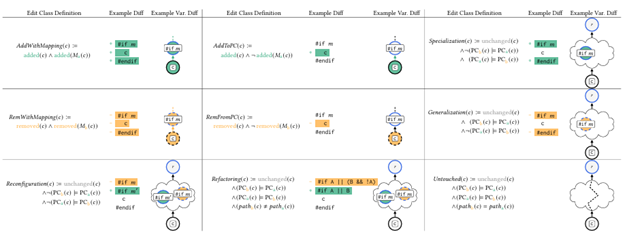
\includegraphics[width=0.9\linewidth]{figures/bittner_edits_classification}
  \caption{Classification of edits to configurable software proposed by Bittner et al.~(2022).}
  \label{fig:bittner_edits}
\end{figure}

At a high level, edits are categorised according to whether they add, remove, or modify variability. The classification distinguishes edits that introduce or delete code together with variability information from those that change the presence conditions of existing code without modifying the code itself.

The classification defines eight fundamental edit categories. Additive edits include \textbf{AddWithMapping}, which describes the addition of new code together with a new presence condition, and \textbf{AddToPC}, which captures additions of code that reuse an existing presence condition. Subtractive edits include \textbf{RemWithMapping} and \textbf{RemFromPC}, which describe different forms of code removal with respect to variability annotations.

More subtle edits affect the variability of unchanged code. A \textbf{Generalization} makes a presence condition less restrictive, increasing the number of configurations in which code is included, while a \textbf{Specialization} makes a presence condition more restrictive. A \textbf{Reconfiguration} replaces a presence condition with a non-comparable alternative, leading to a non-monotonic change in the configuration space. Finally, \textbf{Refactoring} changes the syntactic structure of a presence condition while preserving its semantics.

A key contribution of this classification is that it is complete and unambiguous: every variability-related edit can be assigned to exactly one category. Traditional line-based diff tools cannot capture these distinctions, as they ignore the semantics of presence conditions. The classification therefore provides a necessary abstraction for tools such as \textbf{DiffDetective} and for the analysis performed in this thesis.

\section{Principles of Natural Language Processing}

\subsection{Basics}

% What is the idea behind NLP?
% What techniques can be used to get information of
Natural Language Processing (NLP) is a subfield of computer science and artificial intelligence that focuses on the automatic analysis of human language. The central idea behind NLP is to transform unstructured text into representations that can be processed, analysed, and compared computationally. In software engineering research, NLP is commonly applied to textual artefacts such as commit messages, issue reports, and documentation.

While tools such as DiffDetective make variability-related edits explicit at the code level, commit messages remain a primary source for understanding why such edits were performed. NLP provides a systematic way to analyse these messages across large commit histories.

Despite its usefulness, NLP has inherent limitations. Commit messages are often short, informal, and inconsistent, and may omit important information. As a result, NLP-based analyses should be used as a complementary technique alongside code-based analyses.


\subsection{Topic Modeling}
While DiffDetective identifies how presence conditions change at the source-code level, topic modelling is used to analyse commit messages in order to understand the contexts and intentions under which these changes were made. Topic modelling is an unsupervised NLP technique that discovers underlying thematic structures in a collection of documents.

One of the most widely used topic modelling techniques is \textbf{Latent Dirichlet Allocation (LDA)}, a probabilistic generative model that represents documents as mixtures of topics. In this thesis, topic modelling is applied to commit messages associated with edits to presence conditions identified by \textbf{DiffDetective} and \texttt{MyAnalysis}. Each commit message is treated as a document, and the resulting topics capture recurring themes in developer communication related to variability changes, such as bug fixing, cleanup of conditional compilation directives or refactoring and reconfiguration edits to presence conditions.
	  	\chapter{Implementation}
\label{chp:implementation}



\section{Preliminaries}
% what language structures do you support?
% what tools/libraries help you to achieve your implementation?

\subsection{DiffDetective}

\section{Architecture}
% how is the implementation structured?
% wHat is specific about your implementation?

% ... maybe other sections

% How do we know the implementation is correct?

	  	\section{Evaluation}

\subsection{Setup}
% What repositories have you examined?

\subsection{Results}
% What were the results

\subsection{Threats to Validity}
\cite{Wohlin2024_experimentationInSE}


% 
\chapter{Discussion}
%either we have discussion as chapter or as section of the evaluation both is find and depends a little on the amount of content we have to discuss

% discussion what did go well, what not so well...
	  	
\chapter{Conclusion}
% summarize shortly what you have done in the project
% What is now better than before?
% What are the lessons learned?
% How could we build on that work?
	\endgroup
  	
  	\appendix
  	\listoffigures
  	\listoftables
  	
%    \printglossary[type=\acronymtype]
%    \printglossary
    \printbibliography
\end{document}
